\chapter{Rastreamento Ocular}

\section{Anatomia Ocular}
O globo ocular é majoritariamente opaco, com exceção da córnea, que é transparente. 
A pupila é a região que da passagem para a luz e possui diâmetro variável. Os músculos da íris são os que controlam a dilatação da pupila. 
A focalização da imagem deve se concentrar na fóvea, onde se encontram células muito sensíveis a luz (Helene e Helene, 2011). 
A fixação ocular compreende a um período de cerca de 100 milissegundos onde o olhar se fixa em um ponto de convergência (Barreto et al., 2012). 
Este período se encerra com o movimento de sacada, que compreende ao movimento rápido até uma nova fixação do olhar em outro local.
Através da coleta do posicionamento ocular, é possível calcular uma taxa de dispersão focal ao longo do tempo e piscadas. 
Estes dados foram previamente correlacionados com estados emocionais (Soleymani et al., 2012) e 
também aplicados em estudos com algoritmos de aprendizado de máquina e \textit{deep learning}. 

\begin{figure}[h]
    \centering
    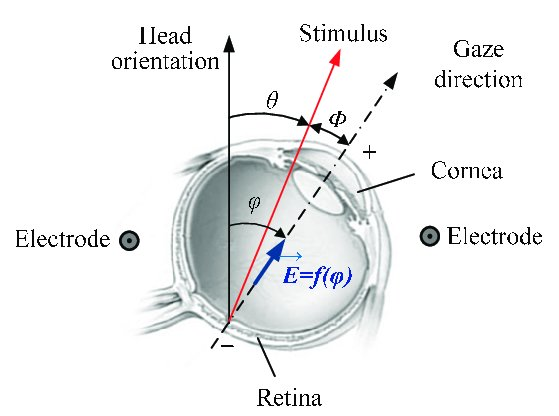
\includegraphics[width=100mm]{Eyeball-modelled-as-a-dipole-and-angular-deviation-of-the-eye-movements-in-response-to-a_W640.jpeg}
    \caption[]{Representação de polaridades no olho humano. Fonte:  López et al. (2019)}\label{fig:}
    \end{figure}

\section{Equipamentos de Rastreamento}
Para detectar onde o participante está focando seu olhar ao longo do tempo, alguns equipamentos de ET
 fazem uso de luz infravermelha e câmeras de alta definição que projetam a luz
  diretamente no olho do participante e gravam a direção do olhar a partir do reflexo. 
  Como a luz infravermelha abrange um comprimento de onda não detectável pelo olho humano, 
  o direcionamento desta luz no olho não interfere visão do participante. 
  O cálculo do direcionamento ocular é feito com base em algoritmos próprios de cada fabricante. 
  Existem alguns tipos de equipamentos de rastreamento ocular. São eles: (1) Webcam, (2) Vestível (Werable) e (3) Baseados em Tela. 
  Webcam diz respeito a equipamentos não especializados para o uso de rastreamento; usáveis correspondem a equipamentos como óculos de rastreamento ocular 
  e realidade virtual, e os baseados em tela dizem respeito aos equipamentos de coleta especializada que podem 
  ser acoplados a um computador (Tobii, 2020).


  \section{Eletrooculograma} 
%Fonte: https://eyewiki.aao.org/Electrooculogram


Também é possível detectar a movimentação ocular através de registros elétricos
no exame de EEG. Isto ocorre devido às características elétricas do olho, que se
comporta como um dipolo (possui duas cargas diferentes separadas), com a córnea
sendo o polo positivo a retina o negativo (López et al., 2019). Isto faz com que seja possível capturar a
movimentação ocular ao colocar os eletrodos próximos aos olhos, como na figura 2.6.
É possível observar picos de voltagem positiva identificados por eletrodos colocados
na posição vertical e picos negativos e positivos identificados por eletrodos na posição
horizontal, acompanhando movimentos de sacada do participante.

A diferença de potencial entre regiões é chamado de \textit{stading potential}, que mede a diferença entre o potencial de membrana da base e topo 
do epitélio de pigmento da retina (Ramkumar et al., 2022).



\begin{figure}[h]
  \centering
  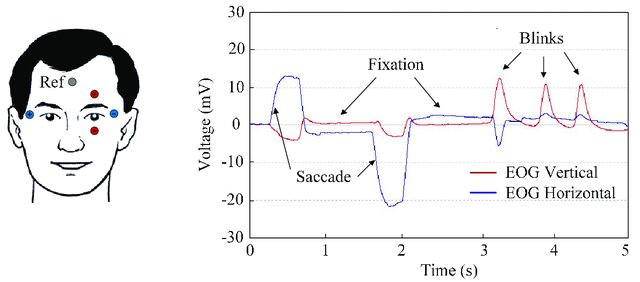
\includegraphics[width=100mm]{EOG-showing-saccadic-and-fixation-eye-movements-as-well-as-blinks-Red-and-blue-waveforms_W640.jpeg}
  \caption[]{Representação de polaridades no olho humano. Fonte:  López et al. (2019)}\label{fig:}
  \end{figure}

  
  
  
